\subsection{Histogram Intersection}
Ein robusteres, aber auch rechenaufwendigeres Verfahren ist der Histogram
Intersection Algorithmus von Swain und Ballard. Farbhistogramme sind stabil
gegenüber Spiegelungen, Verschiebungen und leichten Rotationen um die
Betrachtungsachse (siehe Abbildung \ref{fig:hintersection}). Außerdem ändern sie
sich bei Änderungen des Blickwinkels, des Maßstabs und bei Verdeckung von
Elementen nur langsam. Gegen Belichtungsänderungen können stark reduzierte
Farbhistogramme jedoch Probleme bereiten. \parencite{histogram-swain-ballard}

Im Standardfall wird die Histogram Intersection auf Farbhistogramme angewandt. 
Zuerst muss die Menge an zu diskretisierenden Farben im Histogramm festgelegt
werden - zum Beispiel 200. Folglich gibt es 200 mögliche \glqq{}Farbeimer\grqq{}
(Bins) in die jeder Pixel der Bilder einsortiert wird. Nach dem
Übereinanderlegen der durch das Referenz- und das Suchbild berechneten
Histogrammen, wird schließlich deren Überschneidung berechnet. Je stärker sich
die Histogramme überschneiden, desto ähnlicher sind die Bilder
\parencite{histogram-image-similarity}. Zusätzlich wird wie beim Hashing ein
gewisser Schwellenwert vorher definiert. Der Vorgang kann beispielsweise auch
auf die einzelnen Farbkanäle aufgeteilt werden. Bei RGB würde das bedeuten, dass
man jeweils den Rot-, Grün-, und Blau-Kanal einzeln betrachtet.
\parencite{histogram-swain-ballard}

Eine weitere Untersuchung hat ergeben, dass sowohl die Wahl des Farbraums als
auch die Festlegung des Quantization Levels (Anzahl der Bins) eine große Rolle
bei der Erfolgsschance dieses Vorgehensmodells spielen. In dieser Studie
lieferte der CIELab-Farbraum im Allgemeinen die besten Ergebnisse.
\parencite{histogram-image-similarity}

Um die Genauigkeit des Algorithmus zusätzlich zu verbessern, können neben
Farbhistogrammen weitere Histogramme erstellt und verglichen werden. Ein
mögliches Beispiel wäre ein \glqq{}Texture Direction\grqq{} oder
\glqq{}Texture Scale\grqq{} Histogramm. In diesen Fällen wird nicht versucht
anhand der Farben eine Ähnlichkeit zu erkennen, sondern durch die Struktur des
Bildes. Hier werden beispielsweise aus dem Bild extrahierte Ecken oder Kanten in
ein Histogramm sortiert und schließlich auf Überschneidungen analysiert
\parencite{histogram-stackoverflow}. Natürlich wird jedoch jeder weitere
zusätzlicher Berechnungsschritt die allgemeine Performance des Systems
beeinträchtigen.

\begin{figure}[H]
    \centering
    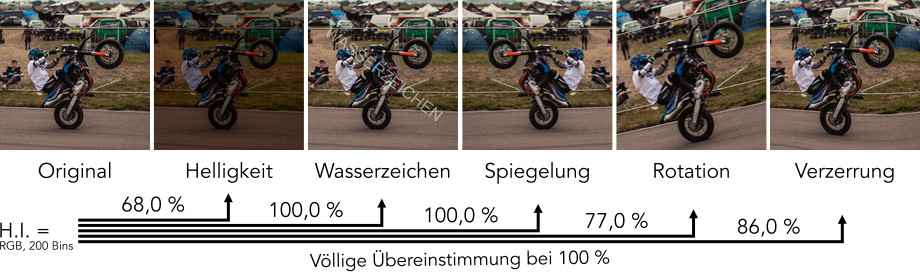
\includegraphics[width=\textwidth]{histogram-intersection}
    \caption{Histogram Intersection: Anwendung an verschiedenen Testbildern}
    \label{fig:hintersection}
    \bildquelle{Eigene Darstellung}
\end{figure}